\documentclass[10pt,portuguese]{article}

\usepackage{fourier}

\usepackage[]{graphicx}
\usepackage[]{color}
\usepackage{xcolor}
\usepackage{alltt}
\usepackage{listings}
\usepackage[T1]{fontenc}
\usepackage[utf8]{inputenc}
\setlength{\parskip}{\smallskipamount}
\setlength{\parindent}{5ex}
\usepackage{indentfirst}
\usepackage{listings}
\usepackage{setspace}
\usepackage{hyperref}
\definecolor{blue(munsell)}{rgb}{0.0, 0.5, 0.69}
\hypersetup{
    colorlinks=true,
    linkcolor=auburn,
    filecolor=magenta,      
    urlcolor=blue, urlsize=2em
}

% Set page margins
\usepackage[top=100pt,bottom=100pt,left=68pt,right=66pt]{geometry}

% Package used for placeholder text
\usepackage{lipsum}

% Prevents LaTeX from filling out a page to the bottom
\raggedbottom


\usepackage{fancyhdr}
\fancyhf{} 
\fancyfoot[C]{\thepage}
\renewcommand{\headrulewidth}{0pt} 
\pagestyle{fancy}

\usepackage{titlesec}
\titleformat{\chapter}
   {\normalfont\LARGE\bfseries}{\thechapter.}{1em}{}
\titlespacing{\chapter}{0pt}{50pt}{2\baselineskip}

\usepackage{float}
\floatstyle{plaintop}
\restylefloat{table}

\usepackage[tableposition=top]{caption}



\frontmatter

\definecolor{light-gray}{gray}{0.95}

\renewcommand{\contentsname}{Table of Contents}

\begin{document}

\selectlanguage{portuguese}

\begin{titlepage}
	\clearpage\thispagestyle{empty}
	\centering
	\vspace{2cm}

	
	{\Large\underline{Computação Distribuída} \par}
	\vspace{0.5cm}
	{\small
	Diogo Nuno Pereira Gomes \par José Nuno Panelas Nunes Lau  \par}
	\vspace{4cm}
	{\LARGE \textbf{Message Broker}} \\
		\vspace{0.5cm}
	\vspace{1cm}
	\vspace{4cm}
	{\normalsize Hugo Paiva, 93195
	        \\Carolina Araújo, 93248
	   \par}
	\vspace{2cm}

    
\includegraphics[scale=0.20]{logo_ua.png}
    
    \vspace{2cm}
    
	{\normalsize DETI \\ 
		Universidade de Aveiro \par}
		
	{\normalsize 22-04-2020 \par}
	\vspace{2cm}
		
	
	\pagebreak

\end{titlepage}
\newpage

\section{Introdução}

\par Este trabalho prático foi desenvolvido com o objetivo de implementar um \textit{Message Broker} capaz de interligar produtores (\textit{Producers}) e consumidores (\textit{Consumers}) através de um protocolo \textit{PubSub} comum e de três mecanismos de serialização distintos (\textit{XML}, \textit{JSON} e \textit{Pickle}). Foi também desenvolvido um \textit{Middleware} para abstrair os produtores e consumidores de todo o processo de comunicação.


\section{Protocolo}

\par Todas as mensagens enviadas são enviadas através do protocolo \textit{TCP} na porta 8000 e precedidas de um \textit{header} que informa ao recetor qual o número de \textit{bytes} que a mensagem terá. Esta metodologia é crucial para a comunicação entre as várias entidades do trabalho prático pois permite receber sempre a mensagem na sua integridade. Seria possível, também, enviar a mensagem com separadores, no entanto o grupo preferiu a abordagem do \textit{header} devido à flexibilidade que permite ter quanto ao tamanho da mensagem.

\par Foi definido que todos os produtores e consumidores, ao inicializarem a respetiva \textit{queue}, enviam uma mensagem ao \textit{Message Broker} com o mecanismo de serialização que suportam. Esta mensagem inicial é codificada em \textit{utf-8} com o nome do mecanismo de serialização em texto simples. Apesar de ser possível enviar a mensagem inicial num mecanismo específico, como \textit{XML}, \textit{JSON} ou \textit{Pickle}, foi escolhida esta abordagem pois desta forma evita-se qualquer tipo de incompatibilidade entre a comunicação das duas entidades, para além do facto de não ser necessário qualquer tipo de operação extra para a descodificação. Ao receber esta mensagem, o \textit{Message Broker} guarda, para cada conexão diferente, o seu respetivo mecanismo de serialização.

\par Após esta mensagem inicial, todos os consumidores e produtores comunicam com o \textit{Message Broker} através do seu mecanismo de serialização específico, tal como pedido no enunciado do trabalho. Em cada mensagem posteriormente enviada, é definida uma operação (\textit{op}), um tópico (\textit{topic}) e um valor (\textit{value}) para representar o que é pretendido enviar.


\section{Estruturas de dados}
\subsection{Tree}
Foi criada uma classe \textit{Tree} com o objetivo de implementar uma árvore hierárquica para os vários tópicos hierárquicos, onde cada instância desta classe representa um nó da mesma. Estas instâncias contêm os seguintes dados:
\begin{itemize}

 \item \textbf{Path} - Tópico completo deste nó, desde a raiz até ao tópico do nó em si;
 
 \item \textbf{Topic} - Último subtópico do \textit{path} completo do nó. Seja o path de um dado nó \textit{/weather/temperature/degree}, o tópico a ele associado sera apenas \textit{degree};
 
\item \textbf{Last\_msg} - Última mensagem que foi produzida para o tópico deste nó;

\item \textbf{Consumers} - Lista de consumidores subscritos ao tópico deste nó; 

\item \textbf{Children} - Lista de todos os nós descendentes diretos;

\item \textbf{Parent} - Guarda, se existir, o nó do qual o próprio provém.

\end{itemize}

\par Foi escolhida esta abordagem quanto à estrutura da árvore porque, visto que um consumer pode estar subscrito a mais do que um tópico, o mais lógico seria instanciar um tipo de estrutura de dados hierárquica para guardar as diferentes entidades, facilitando a criação das funcionalidades necessárias, em vez de tentar colocar tudo numa estrutura como dicionários, listas, etc.

\par Com esta estrutura é-nos possível percorrer a árvore com o intuito de, por exemplo: encontrar todos os nós (tópicos) a que um consumer está subscrito; procurar, entre filhos de um nó, aquele cujo subtópico corresponde ao argumento passado, o que, por sua vez, permite percorrer a árvore entrando apenas nos nós sucessivos descritos por um \textit{path}. Torna-se ainda viável retornar todos os tópicos que têm início no nó em questão, bem como listar todas as últimas mensagens associadas a um tópico que, tendo descendentes, serão também estas listadas, etc.

\par Dito isto, havendo um tópico de onde brotam vários outros, pressupõe-se que, aquando a publicação de novas mensagens nesse tópico-pai, todos os consumers subscritos aos nós-descendentes do mesmo, têm de receber essas novas publicações. Assim sendo, escolheu-se adicionar os consumers do tópico do nó-pai, apenas nesse nó, e remover qualquer subscrição nos nós-descendentes. Isto foi feito com o objetivo de diminuir os tempos de procura ao longo da árvore.

\subsection{Message Broker}
\par O Broker foi construído de modo a controlar o acesso à informação guardada na árvore, utilizando, para o efeito, uma lista que contém a \textit{root} de cada \textit{tree branch} dos vários tópicos, devido às vantagens mencionadas anteriormente.

\par Por outro lado, o \textit{Message Broker} usa um \textit{deque} que guarda os consumidores e produtores que esperam ser atendidos. Desta forma, evitam-se problemas de consistência de dados ao longo da executação dos vários pedidos, uma vez que os pedidos são executados na ordem de chegada e um a um. Apesar de se poder usar outro tipo de resoluções, como um mecanismo de \textit{mutex}, foi escolhida a utilização de um \textit{deque} por ser mais prático e simples. Para evitar erros relativamente ao envio de mensagens para consumidores que entretanto já não estão ativos, sempre que alguma conexão termina, são removidas todas as entradas no \textit{deque} que a contém. Visto que existe uma instância diferente da classe \textit{Queue} para cada produtor e consumidor, fez, também, mais sentido aplicar uma abordagem deste género no \textit{Message Broker} em vez, de por exemplo, um mecanismo de \textit{queue} na classe \textit{Queue}.

\par Por fim, são guardados os mecanismos de serialização de cada conexão num dicionário devido ao fácil e rápido acesso que este tipo de estrutura de dados providencia. 

\clearpage

\section{Arquitetura de Software}
\begin{figure}[!h]
    \centering
    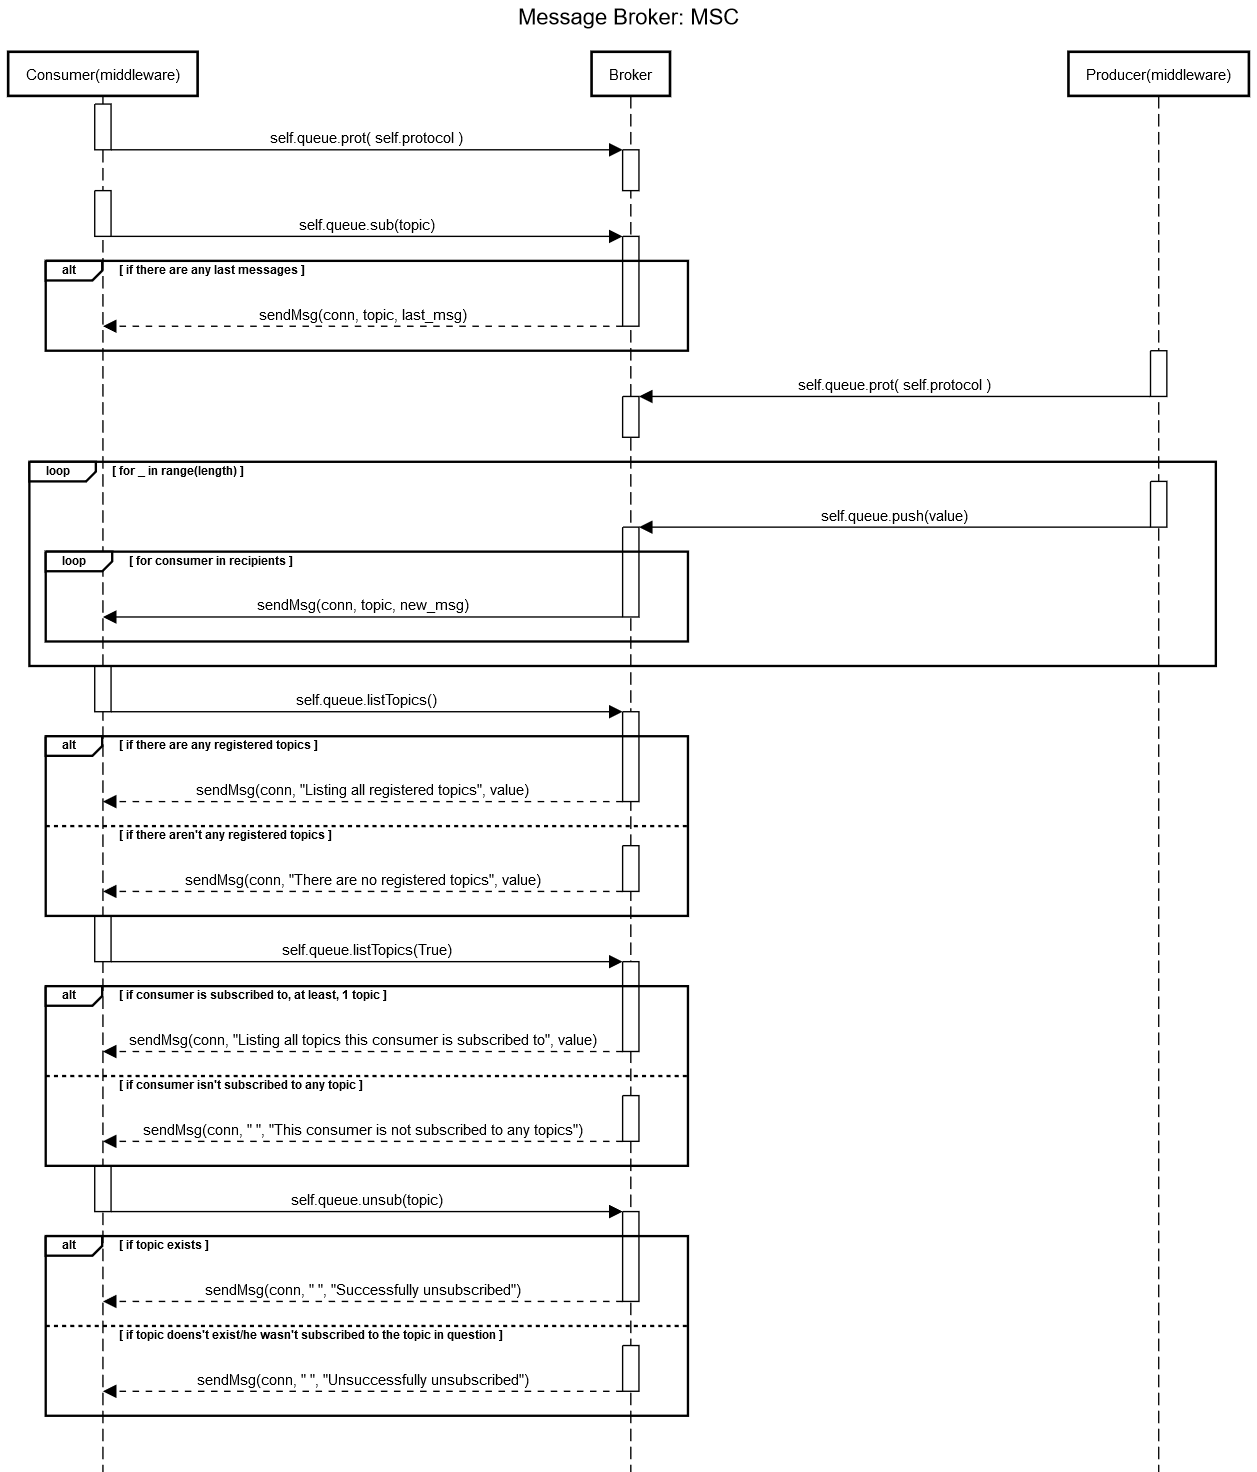
\includegraphics[width=400]{mscMB.png}
\end{figure}

\par Ao serem executados, tanto um consumidor como um produtor criam uma nova instância da classe \textit{Queue} para comunicar com o \textit{Message Broker}, tal como referido na secção do Protocolo.

\par A figura acima representa o fluxo principal de mensagens do trabalho prático realizado. Resumidamente, tanto os \textit{Consumers} como os \textit{Producers} indicam inicialmente o seu protocolo ao \textit{Message Broker}, havendo distinção no facto de apenas os \textit{Consumers} fazerem, logo de seguida, uma ou mais subscrições em tópicos através da função \textit{sub(topic)}.

\par Para a publicação de mensagens, um \textit{Producer} utiliza a função \textit{push(value)}, enviando os vários valores gerados na(s) sua(s) queue(s). Acrescentaram-se  ainda as mensagens de listagem de tópicos e cancelmento de subscrições, por parte dos \textit{Consumers}, para ser possível ver, de modo simplificado, quais as particularidades destas funções.

\section{Interface de listagem de tópicos e cancelamento de subscrição}
\par Optou-se por criar duas opções de listagem de tópicos: listar todos os tópicos registados no \textit{Message Broker} (\textit{listTopics( )}) ou listar todos os tópicos a que está subscrito o consumer que faz o pedido de listagem (\textit{listTopics(True)}), ambas as funções definidas na classe \textit{Queue}. Esta escolha foi feita porque se considerou que ambos seriam uma mais-valia no que toca à verificação da existência, ou não, de erros.
\par Quanto ao cancelamento de subscrição, novamente foram criadas duas opções, sendo que uma delas cancela a subscrição de um tópico específico (\textit{unsub(topic)}) e a outra cancela a subscrição de todos os tópicos a que o \textit{Consumer} estava previamente inscrito (\textit{unsub(" {\textbackslash}") }), ambas as funções definidas na classe \textit{Queue}. Chegou-se à conclusão de que, se era possível subscrever a todos os tópicos registados no \textit{Broker}, então se poderia, de igual modo, cancelar o registo de todos os tópicos.

\section{Estratégia de Validação da Solução}
\par Para validar se a nossa solução correspondia ao esperado, cada vez que se atingia um milestone, os elementos do grupo corriam o \textit{Message Broker}, seguido tanto de um ou mais \textit{Consumers} ou \textit{Producers}, variando, entre estes dois, aquele que era primeiro iniciado. Eram também alterados, se necessários, os códigos base destas duas entidades, testando assim funções como \textit{sub}, \textit{unsub}, \textit{listTopics()}, etc. Deste modo, foi possível encontrar vários erros e/ou chegar à conclusão de que faltava algo essencial. 
\par A par disso, o grupo criou também, na pasta \textit{Testes}, um script de \textit{BASH} que executa em simultâneo 5 \textit{Consumers} e 5 \textit{Producers} que subscrevem e publicam a tópicos diferentes, testando ainda funcionalidades como \textit{list} e \textit{unsub}. 
\section{Conclusão}
\par Em tom de remate, de acordo com as metas especificadas pelos docentes, pensa-se que o trabalho foi bem sucedido. Uma das dificuldades mais sentidas pelo grupo foi conseguir reunir todos os casos a que a nossa solução pode ser submetida e fazer os possíveis para que esta corresponda ao esperado, o que se pensa ter sido alcançado. Foi particularmente custoso saber que muito do trabalho que foi feito acabou por ter de ser riscado da versão final, exatamente pelo motivo previamente mencionado.
\par Considera-se, também, que este trabalho prático ajudou a aprofundar os conhecimentos sobre o funcionamento de um \textit{Messsage Broker}, bem como adquirir novos conhecimentos relacionados com o mesmo.
    


\end{document}

